\section{Persoalan Knapsack (\textit{Knapsack Problem})}
\label{sec:masalah-knapsack}

Algoritma kriptografi Knapsack, atau sistem Merkle--Hellman, didasarkan pada
persoalan matematika klasik yang dikenal sebagai \textit{Knapsack Problem}.
Nama itu diambil dari bayangan sebuah tas ransel (\textit{knapsack}): seseorang
hendak membawa sekumpulan barang, masing-masing berbobot tertentu, dan harus
memilih barang mana saja yang dimasukkan agar berat totalnya tepat sama dengan
kapasitas tas. Persoalan itu tampak sederhana, tetapi sebagaimana akan
diperlihatkan, tidak ada cara yang diketahui untuk menyelesaikannya dengan cepat
ketika jumlah barangnya bertambah banyak.

Sifat ``sulit untuk dipecahkan'' itulah yang menarik perhatian Merkle dan
Hellman \citep{merkle1978}. Gagasan dasarnya sederhana: bila sebuah pesan dapat
dikodekan sebagai jawaban atas persoalan yang sulit, maka pihak yang tidak
memegang kunci juga harus memecahkan persoalan yang sama untuk memulihkan pesan
itu. Sayangnya, sebagaimana akan terlihat pada akhir bab, gagasan itu tidak
bertahan lama --- tetapi perjalanannya justru mengajarkan sesuatu yang penting
tentang apa yang membuat sebuah sistem kunci-publik layak dipercaya.

\subsection{Definisi Matematika}

Diberikan sebuah kapasitas bobot total $M$ dan sekumpulan $n$ buah objek dengan
bobot $w_1, w_2, \dots, w_n$. Persoalannya adalah menentukan nilai biner
$b_i \in \{0, 1\}$ sedemikian sehingga:

\begin{equation}
M = \sum_{i=1}^{n} b_i w_i = b_1w_1 + b_2w_2 + \dots + b_nw_n .
\label{eq:knapsack-dasar}
\end{equation}

Di mana $b_i = 1$ berarti objek ke-$i$ dimasukkan ke dalam tas
(\textit{knapsack}), dan $b_i = 0$ berarti tidak dimasukkan. Karena setiap
$b_i$ hanya boleh bernilai $0$ atau $1$, persoalan ini juga dikenal sebagai
\textbf{persoalan jumlah himpunan bagian} (\textit{subset sum problem}): kita
mencari himpunan bagian dari $\{w_1, \dots, w_n\}$ yang jumlahnya tepat $M$.

\begin{definition}[Persoalan Knapsack]
\label{def:knapsack}
Diberikan barisan bobot $W = \{w_1, w_2, \dots, w_n\}$ berisi bilangan asli dan
sebuah bilangan asli $M$. \textbf{Persoalan knapsack} adalah persoalan
menemukan vektor biner $(b_1, b_2, \dots, b_n)$ yang memenuhi
$M = \sum_{i=1}^{n} b_i w_i$. Vektor itu disebut \textbf{solusi} bagi pasangan
$(W, M)$, dan bila tidak ada vektor semacam itu, pasangan tersebut dikatakan
\textbf{tidak punya solusi}.
\end{definition}

Perlu segera ditegaskan bahwa tidak setiap pasangan $(W, M)$ punya solusi.
Sebagai contoh sederhana, dengan $W = \{2, 4\}$ tidak ada $M = 1$ yang dapat
dibentuk, sebab jumlah yang mungkin hanyalah $0$, $2$, $4$, dan $6$. Keadaan
itu penting bagi kriptografi, sebab proses dekripsi harus memulihkan pesan
dengan tepat, bukan sekadar menemukan jawaban yang mirip.

\begin{figure}[htbp]
    \centering
    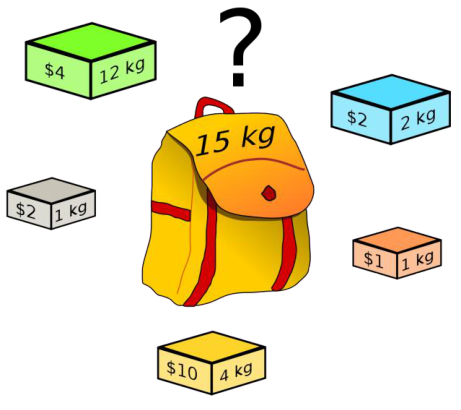
\includegraphics[width=0.75\linewidth, height=0.65\textheight, keepaspectratio]{figures/ilustrasi-masalah-knapsack.png}
    \caption{Ilustrasi masalah knapsack: memilih himpunan barang dengan berat total tepat 15 kg dari sejumlah barang berberat berbeda, persoalan sederhana yang mendasari algoritma knapsack Merkle-Hellman}
    \label{fig:ilustrasi-masalah-knapsack}
    \sumber{Munir, \textit{IF4020 Kriptografi}, ITB.}
\end{figure}

\subsection{Kompleksitas Komputasi}

Cara paling langsung untuk menyelesaikan Persamaan~\eqref{eq:knapsack-dasar}
adalah mencoba seluruh kemungkinan. Karena setiap $b_i$ punya dua nilai, ada
$2^{n}$ vektor biner yang harus diperiksa; untuk $n = 100$ jumlahnya sudah
melebihi $10^{30}$. Cara yang lebih cerdas memang ada --- misalnya dengan
pemrograman dinamik yang berjalan sebanding dengan $M$ --- tetapi biaya itu
tumbuh menurut besar $M$, dan pada pemakaian kriptografis $M$ justru dibuat
sangat besar.

Dalam teori kompleksitas, \textit{Knapsack Problem} umum termasuk dalam kategori
\textbf{NP-complete}. Istilah itu sering disalahpahami, sehingga perlu
dijelaskan dengan tepat. Yang dimaksud bukanlah bahwa persoalan ini mustahil
dipecahkan, melainkan dua hal berikut. Pertama, sekali seseorang menyerahkan
calon solusi $(b_1, \dots, b_n)$, memeriksa apakah jawabannya benar hanya
memerlukan penjumlahan $n$ buah suku --- jadi \emph{pemeriksaannya} berjalan
dalam waktu polinomial. Kedua, meskipun demikian, tidak ada algoritma yang
diketahui dapat \emph{menemukan} solusi itu dalam waktu polinomial; seluruh
algoritma yang diketahui tumbuh eksponensial terhadap $n$. Kata
``diketahui'' itu penting: yang belum ditemukan mungkin saja ada, dan
justru ketidakpastian itulah yang membuat persoalan ini dipakai sebagai
landasan keamanan. Jika suatu hari seseorang menemukan algoritma polinomial
untuk persoalan NP-complete, seluruh keluarga sistem yang bertumpu padanya
runtuh sekaligus.

\subsection{Mengapa Persoalan Sulit Menjadi Landasan Kriptografi}

Gagasan mengubah persoalan ini menjadi sistem kriptografi disusun secara
terbalik dari kebiasaan. Pada kriptografi kunci-simetri, kunci adalah sesuatu
yang harus dibangkitkan lalu dirahasiakan. Pada algoritma knapsack, yang
menjadi kunci rahasia justru \emph{barisan bobot} $w_1, w_2, \dots, w_n$ itu
sendiri, sedangkan pesan diwakili oleh pilihan $b_i$. Dengan kata lain:

\begin{itemize}
    \item Setiap bit plainteks menentukan apakah objek ke-$i$ dimasukkan ke
          dalam tas.
    \item Kriptogramnya adalah berat total tas, yaitu bilangan bulat $M$ pada
          Persamaan~\eqref{eq:knapsack-dasar}.
    \item Pihak yang menyadap kriptogram menerima bilangan $M$ dan harus
          menentukan barang mana saja yang menyusunnya. Untuk barisan bobot yang
          umum, itulah persoalan yang sulit tadi.
\end{itemize}

Namun di sinilah muncul persoalan pertama. Misalkan barisan bobot dirahasiakan.
Penerima pesan yang sah pun tidak dapat mendekripsinya, sebab ia hanya menerima
bilangan $M$ tanpa mengetahui susunan $w_i$ yang mustahil direkonstruksi tanpa
menyelesaikan persoalan NP-complete itu sendiri. Karena itu algoritma knapsack
sederhana hanya dapat \textbf{dipakai untuk enkripsi, tetapi tidak untuk
dekripsi} ---
keadaan yang jelas tidak berguna bagi sistem kunci-publik, sebab penerima harus
mampu membaca pesan yang dikirim kepadanya.

Jalan keluar dari persoalan itu adalah memilih barisan bobot yang \emph{istimewa},
sehingga dekripsi menjadi mudah bagi pemilik rahasia, sementara penyadap tetap
menghadapi persoalan yang sulit. Barisan istimewa itu adalah
\textbf{barisan superincreasing}, yang dibahas pada Bagian~\ref{sec:superincreasing}.
Di antara kedua kutub itulah sistem Merkle--Hellman bekerja.

\subsection{Tiga Varian Persoalan Knapsack}

Ketiga varian itu dirangkum pada Tabel~\ref{tab:varian-knapsack}.

\begin{table}[htbp]
    \centering
    \caption{Tiga varian persoalan knapsack dan perannya}
    \label{tab:varian-knapsack}
    \begin{tabularx}{\linewidth}{@{}>{\raggedright\arraybackslash}p{3.1cm}
                                   >{\raggedright\arraybackslash}p{3.0cm}
                                   >{\raggedright\arraybackslash}X@{}}
    \toprule
    \textbf{Varian} & \textbf{Kesulitan} & \textbf{Peran} \\
    \midrule
    Knapsack dasar & Sulit bagi semua pihak &
    Hanya dapat dipakai untuk enkripsi; penerima yang sah pun tidak dapat
    mendekripsi \\
    \addlinespace
    Superincreasing \newline knapsack & Mudah, $O(n)$ &
    Dapat didekripsi dengan algoritma \textit{greedy}, sehingga tidak layak
    dipakai langsung sebagai sistem kriptografi \\
    \addlinespace
    Non-superincreasing \newline (\textit{knapsack} normal) & Sulit, eksponensial &
    Menjadi wujud kunci publik; barisan superincreasing disembunyikan di
    baliknya \\
    \bottomrule
    \end{tabularx}
\end{table}

Tabel itu memperlihatkan pola yang khas dalam perancangan kriptografi
kunci-publik: yang dicari bukan persoalan yang sulit bagi siapa pun, melainkan
persoalan yang \emph{mudah bagi pemegang kunci} dan sulit bagi yang lain.
Selisih kemampuan itu disebut \textbf{pintu jebakan} (\textit{trapdoor}), dan
pada Merkle--Hellman pintu jebakannya adalah sepasang parameter $(n, m)$ yang
mengubah barisan mudah menjadi barisan yang tampak sulit --- dan sebaliknya,
bila diketahui.
